\section{Design}
\subsection{Architettura}
In fase di progettazione è stato scelto di adottare il pattern architetturale MVC, traendone quindi tutti i suoi vantaggi, principalmente che model e controller rimangono praticamente uguali a prescindere dalla view utilizzata. Infatti, per la view è stato scelto di usare il pattern Strategy con delle interfacce generiche per i singoli componenti che potranno perciò adottare qualsiasi GUI framework. Per passare per esempio da Swing a JavaFX basterebbe solo sostituire le implementazioni delle interfacce presenti nella parte di view.
\medskip

Ogni modulo del pattern Model-View-Controller ha quindi una propria organizzazione e scopo:
\begin{itemize}
    \item Nella parte di model sono state definite le entità che modellano: tessere (tile), seguaci (meeple), strutture (gameset) e giocatori (player). Esse vengono instanziate e gestite dal controller.
    \item Nella parte di view è presente un componente principale, la UserInterface, che si occupa di gestire tutti i componenti grafici e di renderli visibili all'utente quando necessario. Quest'ultima si occupa anche di fornire ai vari componenti, ognuno con uno scopo ben preciso, l'accesso regolarizzato alla parte di controller. Nella maggior parte dei casi questi componenti sono annidati l'uno dentro l'altro.
    \item La parte di controller si occupa della gestione della partita e di propagare sul model i risultati delle azioni compiute dall'utente attraverso la view.
\end{itemize}
Siccome ad ogni modifica di stato della partita, il Controller notifica le UserInterface collegate ad esso, è possibile giocare alla stessa partita contemporaneamente tramite varie interfacce utente aggiungendole tutte allo stesso controller. Queste possono essere diverse tra loro e di qualsiasi tipo, per esempio: Web, CLI o come nel nostro caso, GUI.
\medskip

Per la configurazione iniziale della partita viene utilizzato un file JSON. All'interno di esso vengono memorizzate informazioni riguardo quali e quante tile generare all'inizio della partita e quale deve essere la tile iniziale.

\begin{figure}[hb]
    \centering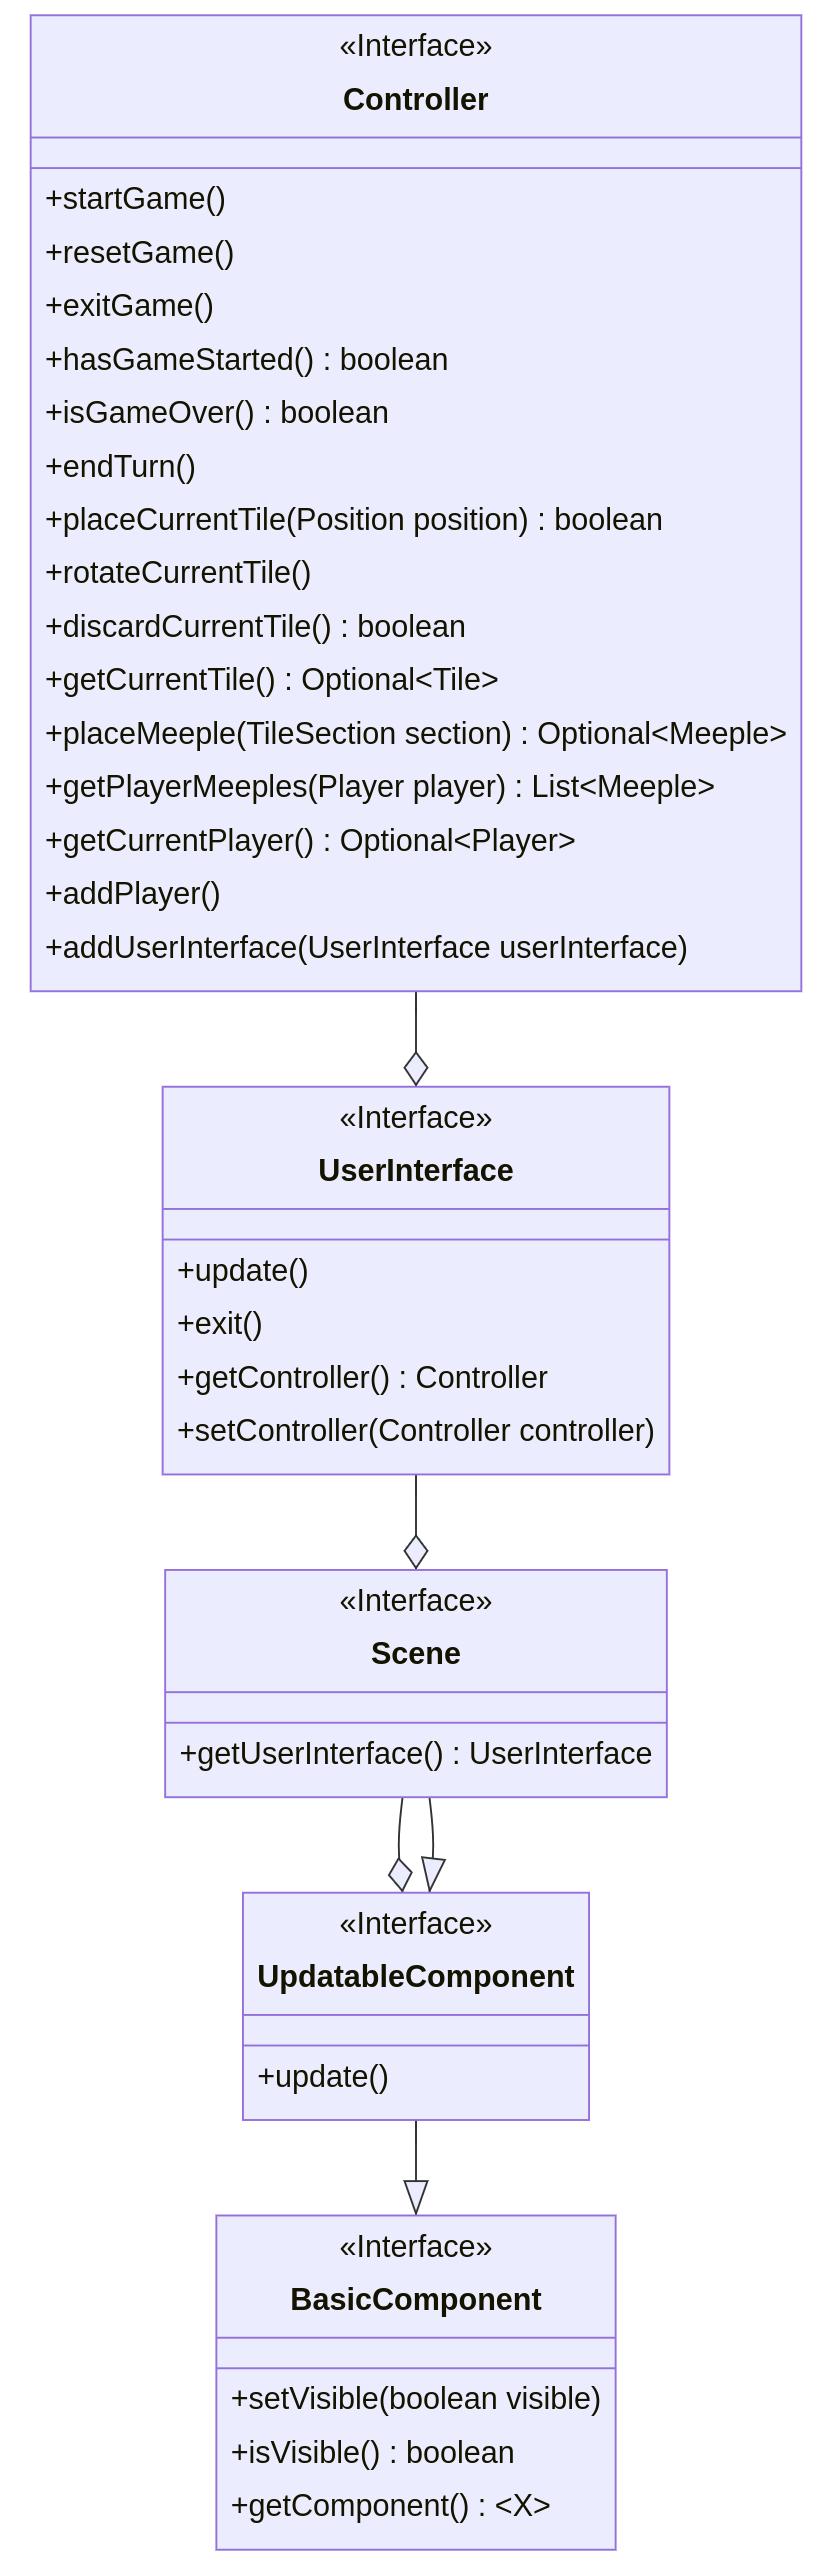
\includegraphics[scale=0.29]{images/design_uml.png}
    \caption{Schema UML architetturale.}
\end{figure}
\clearpage

\subsection{Design dettagliato}
\subsection*{Mauro Pellonara}

\subsubsection*{Permettere di sviluppare Meeple con diverse caratteristiche}
\begin{figure}[ht]
    \centering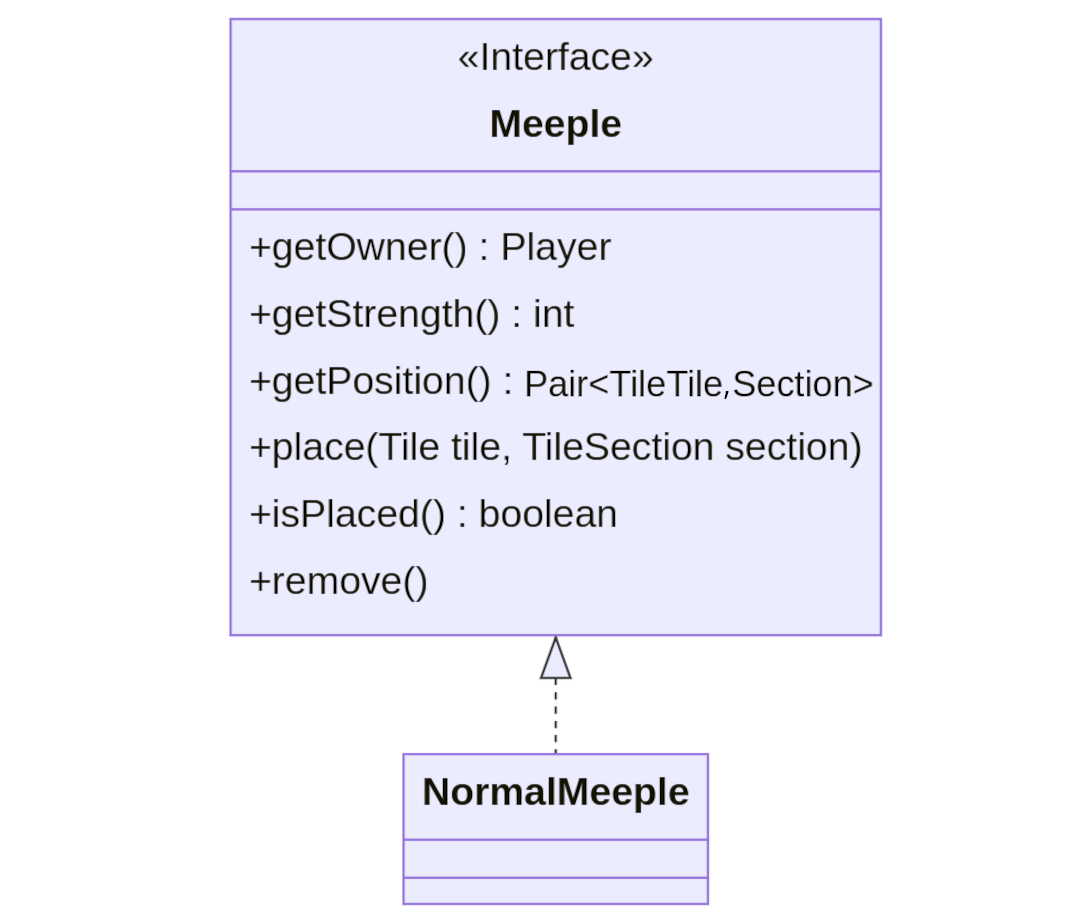
\includegraphics[scale=.25]{images/meeple.png}
    \caption{Rappresentazione UML dell'applicazione del pattern Strategy per Meeple e NormalMeeple.}
\end{figure}
\paragraph{Problema}
La versione classica del gioco supporta solo seguaci normali che non hanno funzioni speciali. Alcune espansioni introducono invece dei seguaci che valgono il doppio di quelli normali, è quindi necessario garantire espandibilità futura in caso di nuove espansioni.
\paragraph{Soluzione}
Usare il pattern Strategy sulla classe NormalMeeple introducendo un'interfaccia Meeple che può essere usata in futuro per introdurre nuovi seguaci di tipo diverso, un esempio sono quelli che hanno valore doppio rispetto ai normali.
\clearpage

\subsubsection*{Facilitare la creazione di istanze di MutableTile assieme ai relativi GameSet}
\begin{figure}[ht]
    \centering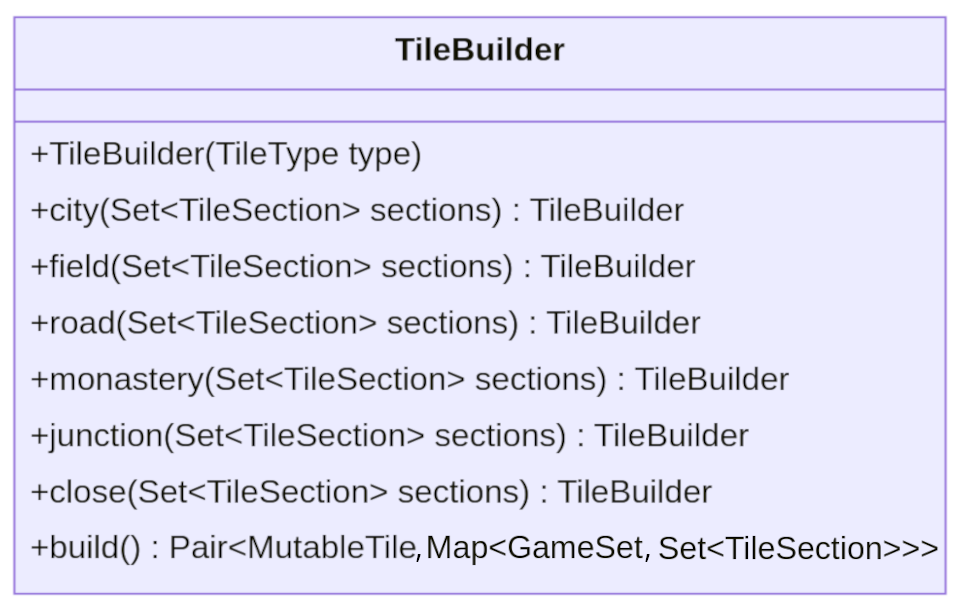
\includegraphics[scale=.30]{images/tilebuilder.png}
    \caption{Rappresentazione UML dell'applicazione del pattern Builder per MutableTile.}
\end{figure}
\paragraph{Problema}
Creare istanze di MutableTile assieme ai relativi GameSet in modo facile e leggibile.
\paragraph{Soluzione}
Usare il pattern Builder per la creazione di oggetti MutableTile rendendo più esplicite le istruzioni da eseguire. Assieme alla creazione di un'istanza di MutableTile possono anche essere creati i relativi GameSet e restituiti tutti assieme con il metodo build().
\clearpage

\subsubsection*{Facilitare la creazione di istanze di MutableTile di tipo diverso}
\begin{figure}[ht]
    \centering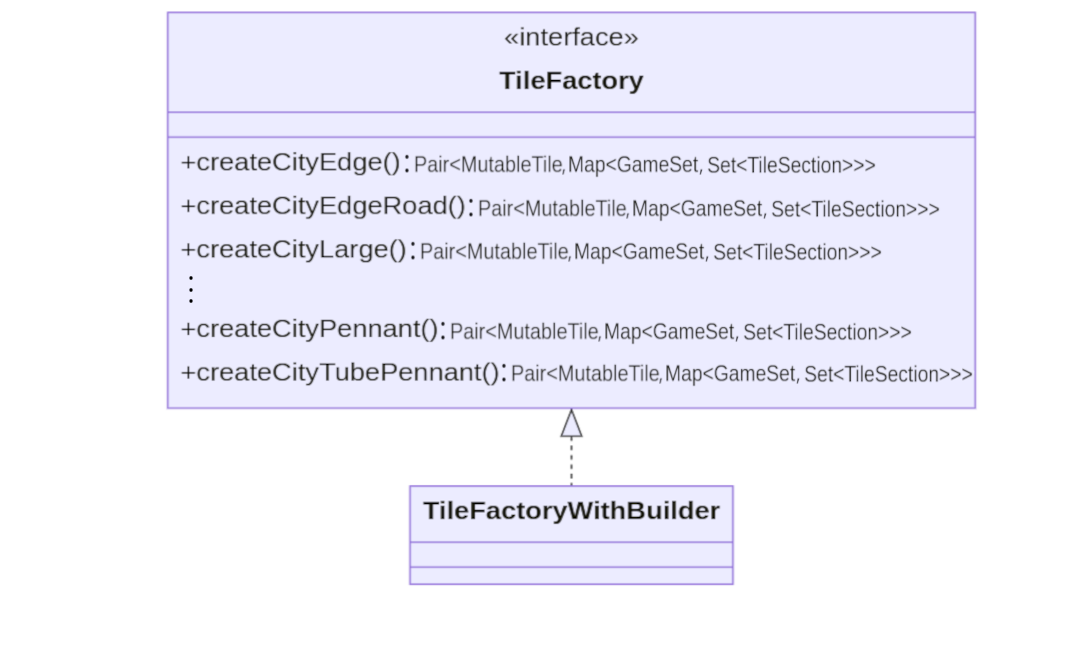
\includegraphics[scale=.35]{images/tilefactory.png}
    \caption{Rappresentazione UML dell'applicazione del pattern Factory Method per MutableTile.}
\end{figure}
\paragraph{Problema}
All'inizio di ogni partita vengono generate numerose MutableTile per ogni tipo rispettando il file di configurazione, è quindi necessario che per ogni tipo di Tile ci sia una procedura facile e ripetibile per la generazione.
\paragraph{Soluzione}
Usare il pattern Factory Method includendo nella classe TileFactoryWithBuilder, per ogni tipo di Tile, un metodo per la creazione di MutableTile di quel tipo. In aggiunta, è stato usato anche il pattern Strategy aggiungendo un'interfaccia per le Factory di MutableTile, in questo modo ogni Factory può impiegare algoritmi e strategie diverse per conseguire lo stesso risultato. In questo caso è stata sviluppata una factory che usasse la classe TileBuilder per la creazione di MutableTile.
\clearpage

\subsubsection*{Evitare di avere riferimenti doppi tra GameSet e Tile}
\begin{figure}[ht]
    \centering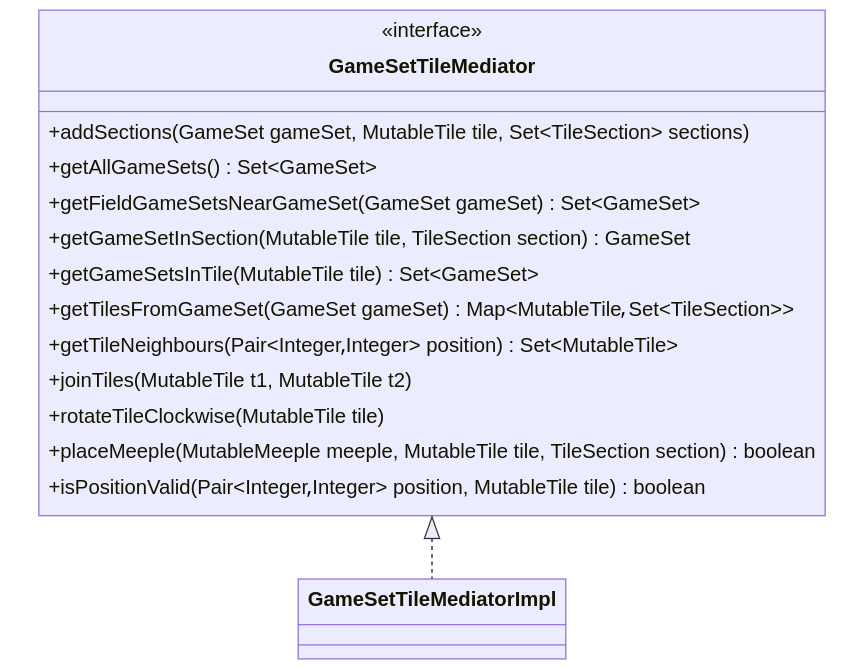
\includegraphics[scale=.35]{images/gamesettilemediator.png}
    \caption{Rappresentazione UML dell'applicazione del pattern Mediator per GameSet e Tile.}
\end{figure}
\paragraph{Problema}
Ogni singola Tile alla sua creazione ha su di essa diversi GameSet. Questi però non esistono solo sulle singole Tile ma riguardano il tabellone di gioco in generale, in quanto, con l'avanzamento progressivo della partita, vengono estesi ed uniti tra loro. Perciò, ogni Tile contiene dei GameSet e ogni GameSet contiene delle Tile, serve quindi un modo di gestire questo legame.
\paragraph{Soluzione}
Usare il pattern Mediator per creare una classe che si occupi del legame tra GameSet e Tile, permettendo quindi di eseguire operazioni come ottenere i GameSet presenti in una Tile o ottenere le Tile sulla quale si estende un certo GameSet. Quindi, usando questo pattern non sarà necessario tenere e sincronizzare dei riferimenti doppi tra GameSet e Tile. In aggiunta, è stato usato anche il pattern Strategy aggiungendo un'interfaccia per il Mediator, in questo modo ognuno può impiegare algoritmi e strategie diverse per conseguire lo stesso risultato.
\clearpage

\subsubsection*{Permettere diversi tipi di campi di input per la creazione di Player}
\begin{figure}[ht]
    \centering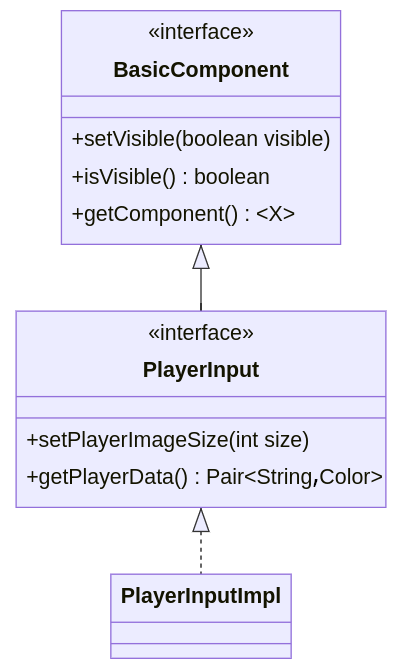
\includegraphics[scale=.35]{images/playerinput.png}
    \caption{Rappresentazione UML dell'applicazione del pattern Strategy per PlayerInput.}
\end{figure}
\paragraph{Problema}
Creare un componente grafico per l'inserimento delle informazioni necessarie alla creazione di un nuovo Player, rispettando quindi il Single Responsibility Principle. In oltre, far si che questo principio venga rispettato da qualsiasi view con interfaccia grafica.
\paragraph{Soluzione}
Creare una classe PlayerInputImpl che si occupi di ottenere e gestire le informazioni relative alla creazione di un nuovo Player. Ulteriormente, applicare il pattern Strategy alla classe PlayerInputImpl generalizzandone il comportamento e usando un tipo generico rappresentante il componente grafico utilizzato, che varia a seconda del GUI framework scelto.
\clearpage

\subsection*{Alessandro Martini}

\subsubsection*{Definizione di operazioni che vengono utilizzati su GameSet differenti}
\begin{figure}[ht]
    \centering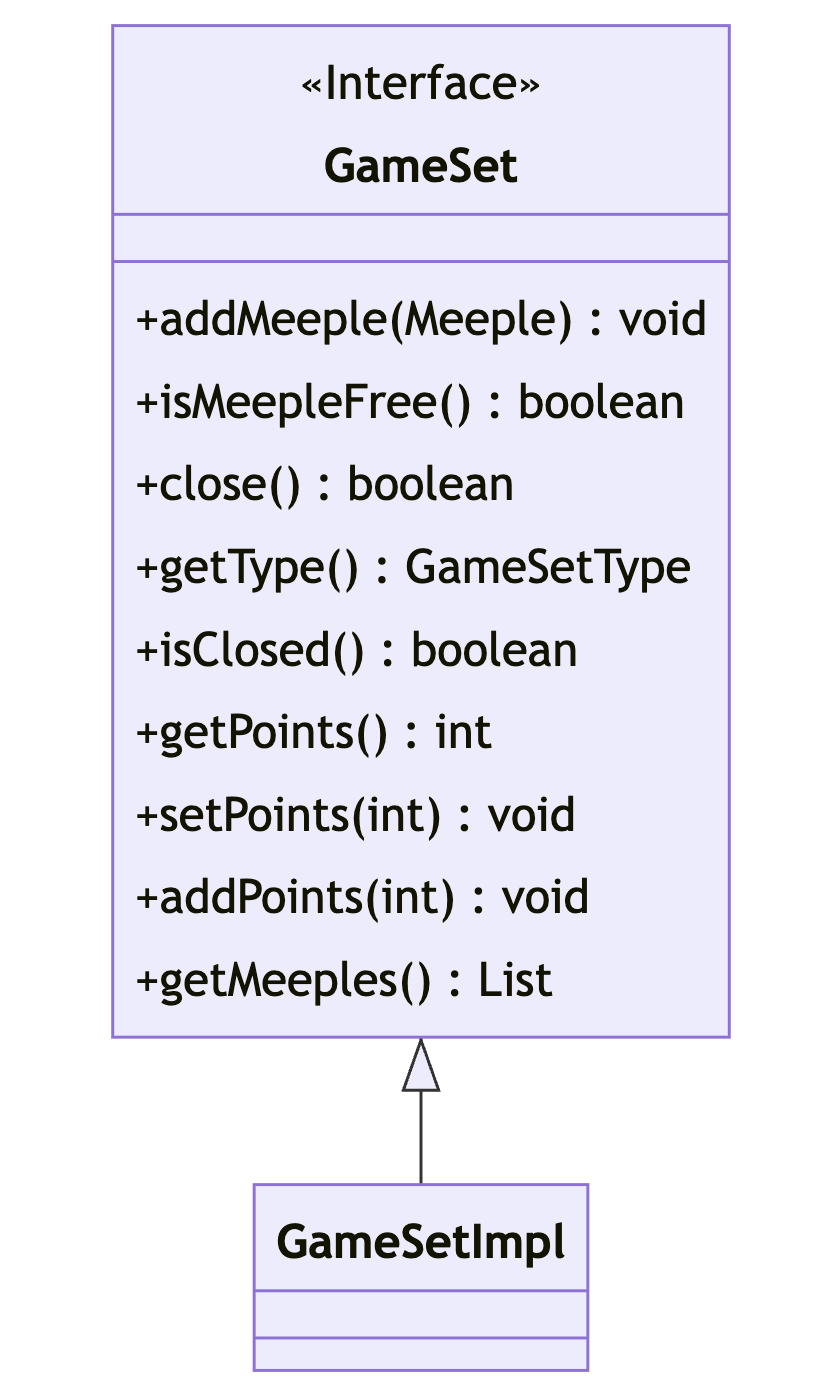
\includegraphics[scale=.4]{images/gameset.png}
    \caption{Rappresentazione UML dell'applicazione del pattern Strategy per GameSet e GameSetImpl}
\end{figure}
\paragraph{Problema:}
Assegnare logiche differenti per GameSet differenti. Si era posto il problema della scalabilità delle funzioni che ogni GameSet dovesse avere, anche per aggiornamenti futuri
\paragraph{Soluzione:}
Tramite il patter Strategy, sono andato a creare un'interfaccia GameSet che definisse le funzioni generali di ogni GameSet, così facendo, ho reso scalabile anche per upgrade futuri la possibilità di creare nuove funzioni e nuove regole per i vari tipi di GameSet.
\clearpage

\subsubsection*{Creazione di più GameSet con tipologie differenti}
\begin{figure}[ht]
    \centering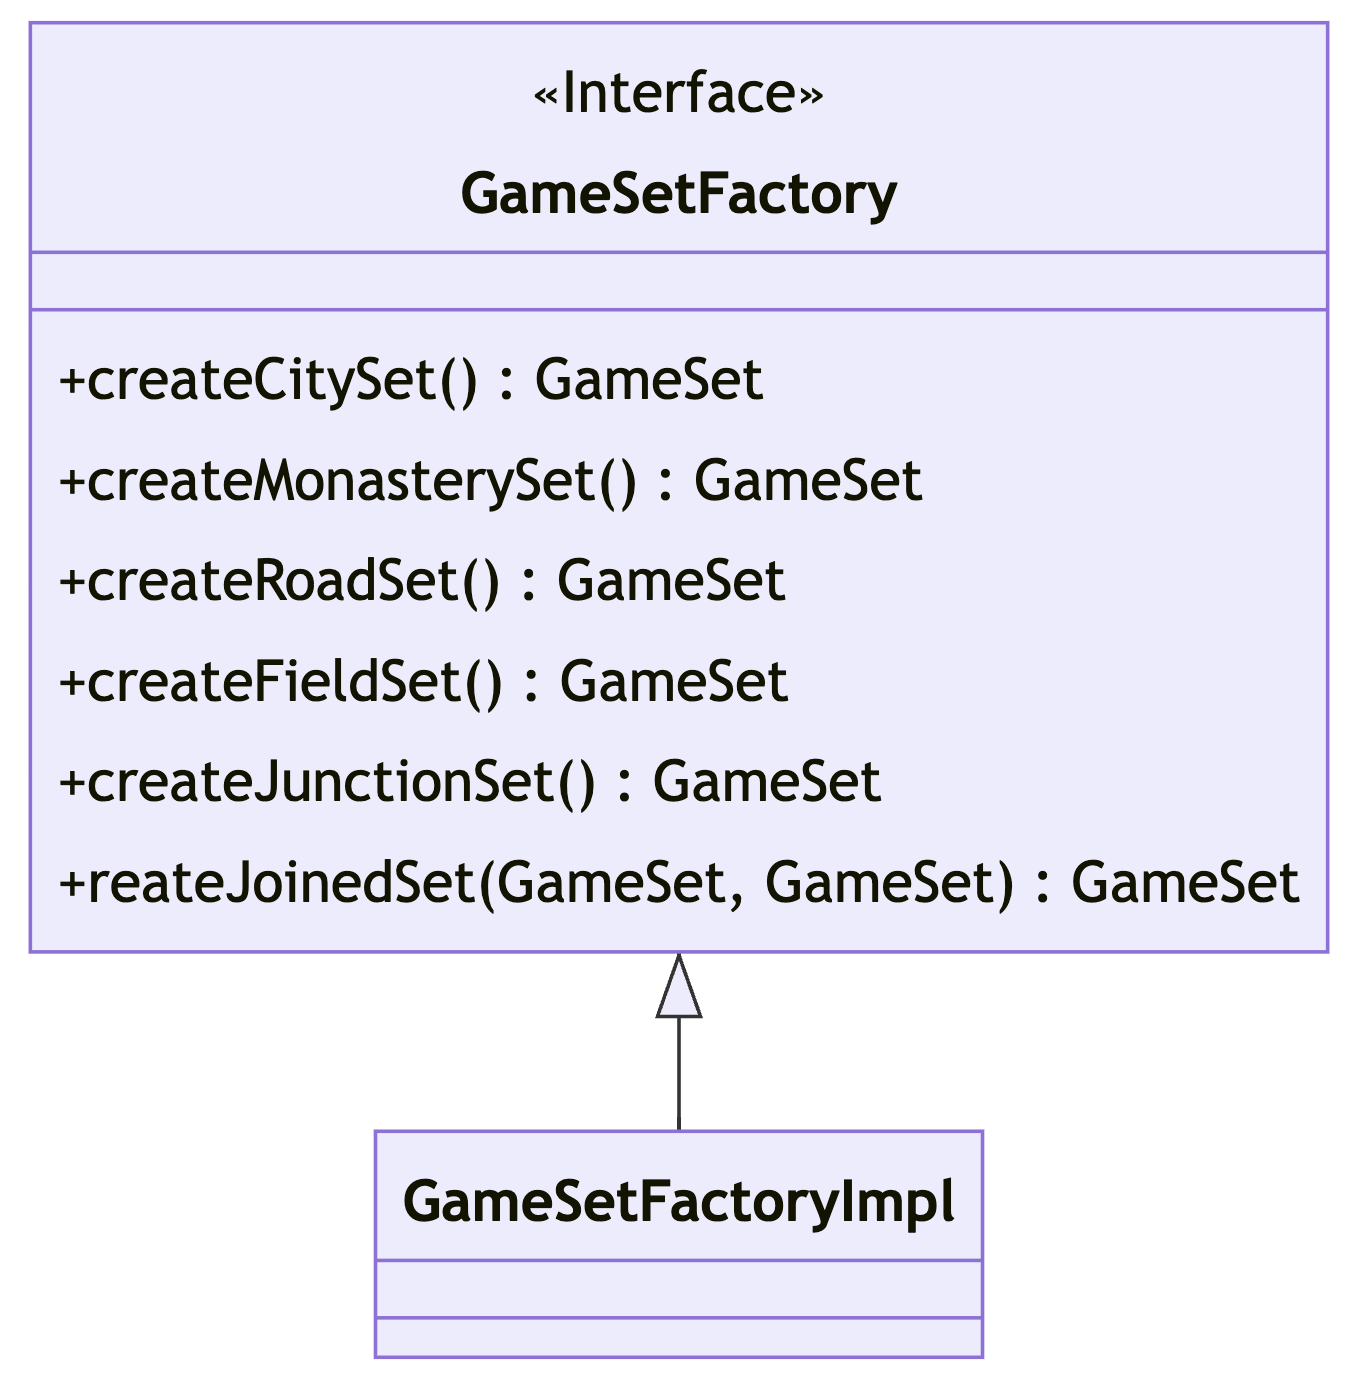
\includegraphics[scale=.3]{images/gamesetfactory.png}
    \caption{Rappresentazione UML dell'applicazione del pattern Strategy per il gamesetfactory e GameSetFactoryImpl}
\end{figure}

\paragraph{Problema:}
Creare una uguale implementazione di GameSet ma di tipi differenti
\paragraph{Soluzione:}
Tramite il pattern Strategy, siamo andati a implementare dei metodi che vanno a definire come i vari tipi di GameSet vengono creati, e inoltre come si possono creare dei GameSet da altri GameSet
\clearpage

\subsubsection*{Creazione di più BasicComponent con caratteristiche differenti}
\begin{figure}[ht]
    \centering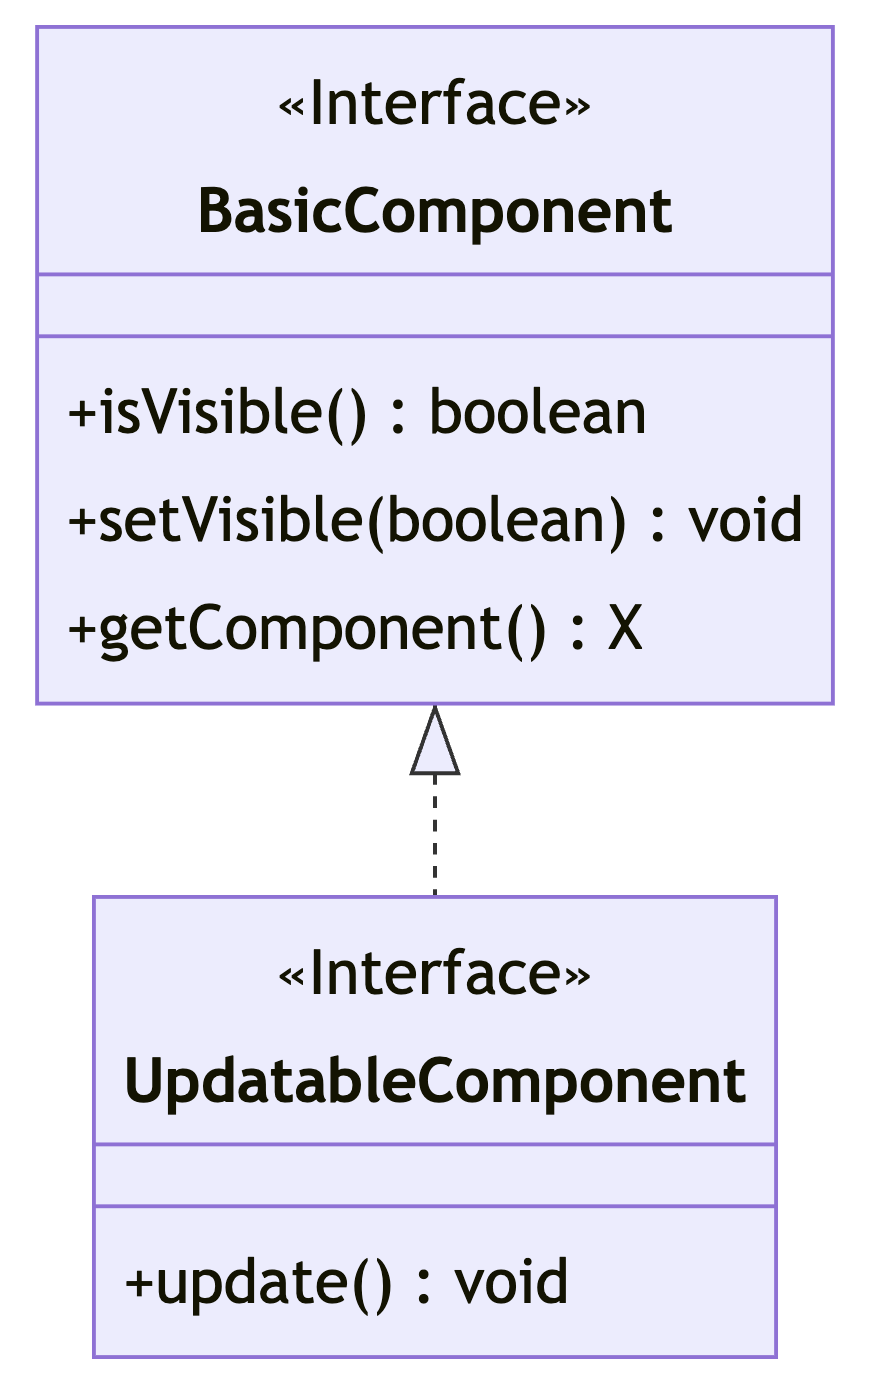
\includegraphics[scale=.3]{images/basiccomponent.png}
    \caption{Rappresentazione UML dell'applicazione del pattern Strategy per la classe interfaccia BasicComponent, che viene estesa dal'interfaccia  UpdatableComponent}
\end{figure}

\paragraph{Problema:}
Erano presenti dei componenti Grafici che, oltre ai metodi in comune con gli altri, avevano necessità di essere aggiornati durante il gioco
\paragraph{Soluzione:}
Sempre tramite il pattern Strategy, sono andato ad implementare i metodi che vanno a definire i comportamenti (metodi) in comune tra i vari componenti della view, e successivamente ho creato un'altra interfaccia che, estende BasicComponent, e inoltre va a definire il comportamento (metodo) di update del componente.
\clearpage

\subsection*{Davide Speziali}


\subsubsection*{Associazione tra View e Model per quanto riguarda le immagini di tasselli e seguaci}
\begin{figure}[h]
    \centering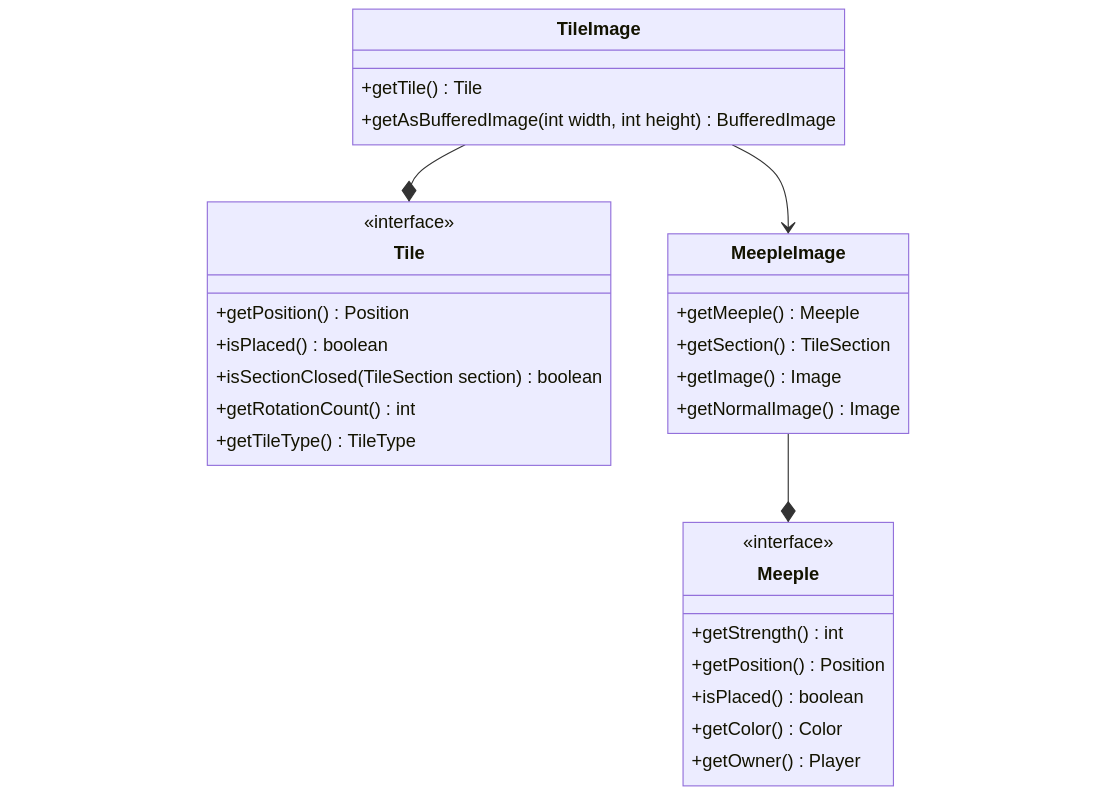
\includegraphics[scale=.4]{images/uml_tilemeeple_images.png}
    \caption{Rappresentazione UML della gestione delle immagini di tile e meeple}
\end{figure}
\paragraph{Problema:}
Necessità di avere delle imamgini aggiornate sulla base dello stato dei singoli tasselli e seguaci presenti nel gioco. Che devono inoltre essere presenti
sia nel footer che nel tabellone.
\paragraph{Soluzione:}
Per quanto riguarda i taselli la soluzione trovata è stata quella di creare una classe TileImage che al suo interno contenesse una referenza ad oggetto della classe Tile. In questo modo viene fatta un'associazione diretta tra ogni singola instanza della classe Tile e la sua immagine, senza necessità che il model sia a conoscenza dell'esistenza di quest'ultima. All'interno di TileImage viene generata un'immagine corrisponendente alla tile che viene rigenerata ogni volta che avviene una modifica: rotazione, piazzamento di meeple o rimozione di meeple. Queste ultime due modifiche vengono gestite attraverso la classe MeepleImage che TileImage usa per ottenere l'overlay dei seguaci da applicare alle immagini dei tasselli. La classe MeepleImage è gestita in maniera analoga a TileImage, contiene e si associa in maniera diretta a un'istanza della classe Meeple. Questo sistema, oltre a garantire la gestione dinamica delle immagici, ci permette di attuare una forma di caching, non essendo necessario generare una nuova immagine ogni qual volta un tassello viene girato o un seguace viene piazzato su di esso. Questa soluzione garantisce che sia MeepleImage che TileImage vengano utilizzati anche indipendentemente.

\subsubsection*{Permettere al giocatore l'utilizzo del tabellone di gioco}
\begin{figure}[h]
    \centering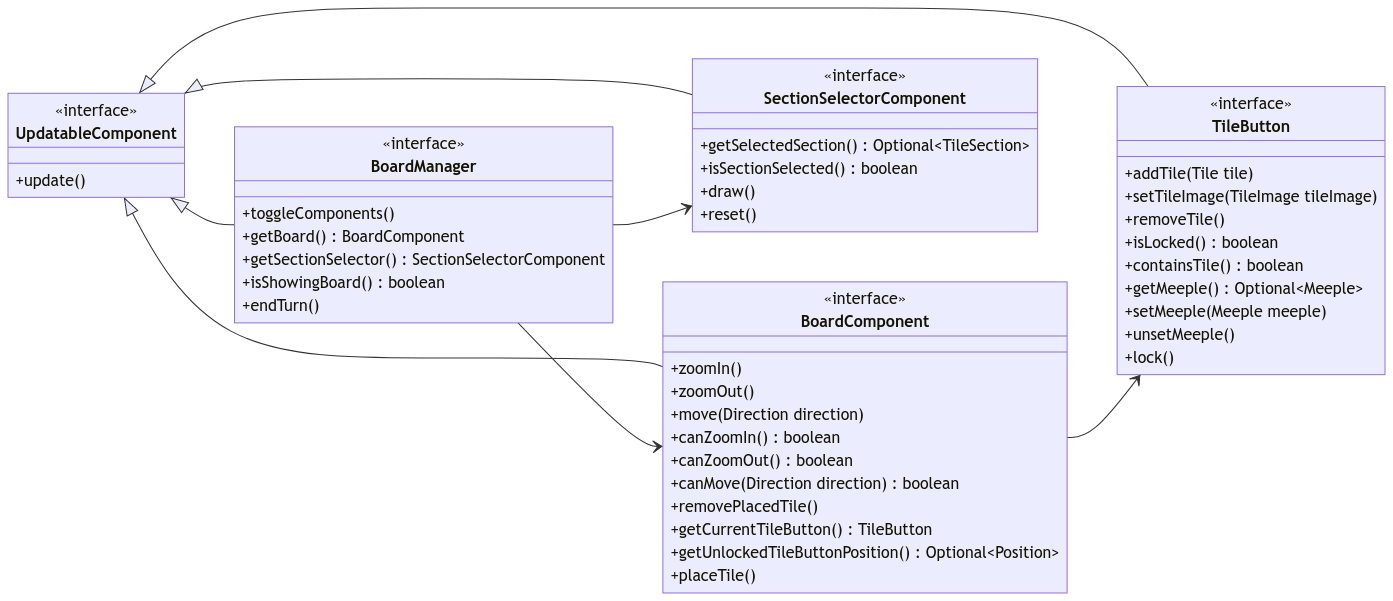
\includegraphics[scale=.3]{images/uml_board.png}
    \caption{Rappresentazione UML della gestione dei componenti grafici del tabellone di gioco}
\end{figure}
\paragraph{Problema:}
È necessaria la creazione di una GUI in grado di permettere al giocatore di:
\begin{itemize}
    \item Posizionare tessere
    \item Posizionare seguaci su tessere appena piazzate
\end{itemize}
\paragraph{Soluzione:}
Per garantire il \textit{single responsability principle} la soluzione trovata è stata quella di creare 4 componenti:
\begin{itemize}
    \item TileButton, rappresenta una posizione nella board, può quindi contenere tasselli e seguaci
    \item BoardComponent, contiene i vari TileButton
    \item SectionSelectorComponent, permette di selezionare dove piazzare esattamente i seguaci
    \item BoardManager, gestisce la visualizzazione alternata tra BoardComponent e SectionSelectorComponent
\end{itemize}
Inoltre per facilitare espandibilità e refactoring è stato utilizzato il pattern \textit{Strategy} per definire le operazioni richieste a ogni componente. Nel mio caso in particolare è stato utilizzato per definire il comportamento di tutti e quattro i componenti sopracitati.

\subsubsection*{Condivisione di elementi del Model nella View}
\begin{figure}[h]
    \centering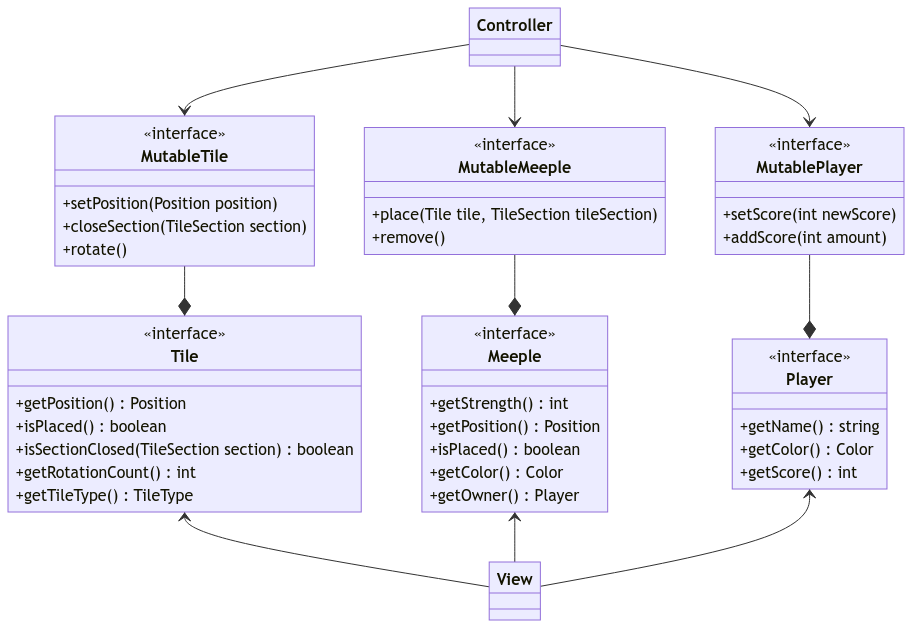
\includegraphics[scale=.4]{images/uml_mutability.png}
    \caption{Rappresentazione UML dei componenti del Model nella gestione della mutabilità}
\end{figure}
\paragraph{Problema: Come gestire la necessità di avere riferimenti a componenti del Model all'interno della View, evitando di dare la possibilità a quest'ultima di apportare modifiche al Model.}
\paragraph{Soluzione:}
La soluzione trovata è stata quella di utilizzare il concetto di \textit{Immutability Through Interfaces}. Esso consiste nell'avere un'interfaccia, contenete soltanto metodi di richiesta di informazioni, che viene estesa dall'ulteriore interfaccia contenente anche medoti che comportano la modifica delle informazioni delle istanze. Le classi implementeranno direttamente questa seconda interfaccia mutabile, la prima interfaccia verrà solo utilizzata come tipo all'interno della View, in modo che quest'ultima abbia accesso ai dati aggiornati riguardo il Model ma allo stesso tempo non possa in nessun modo modificarli.

Questa tecnica è stata utilizzata per le interfacce:
\begin{itemize}
    \item Meeple $\rightarrow$ MutableMeeple
    \item Player $\rightarrow$ MutablePlayer
    \item Tile $\rightarrow$ MutableTile
\end{itemize}

\subsection*{Samuele Giancarli}
\subsubsection*{Definizione di Tile}
\begin{figure}[ht]
    \centering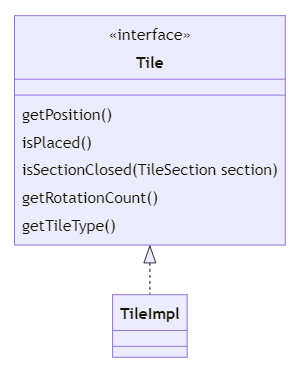
\includegraphics[]{images/tile_uml.png}
    \caption{Rappresentazione UML dell'applicazione del pattern Strategy per Tile.}
\end{figure}
Ogni tile è divisa in sezioni indipendenti (TileSection) ognuna definita dal una tipologia di struttura (GameSet)
\paragraph{Problema:}
Necessità di garantire espandibilità futura, in quanto nuove Tile potrebbero prevedere anche nuove meccaniche di gioco.
\paragraph{Soluzione:}
Usare il pattern Strategy sulla classe TileImpl introducendo un'interfaccia Tile che potrà essere usata in futuro.
\clearpage

\subsubsection*{Gestione della HUD}
\begin{figure}[ht]
    \centering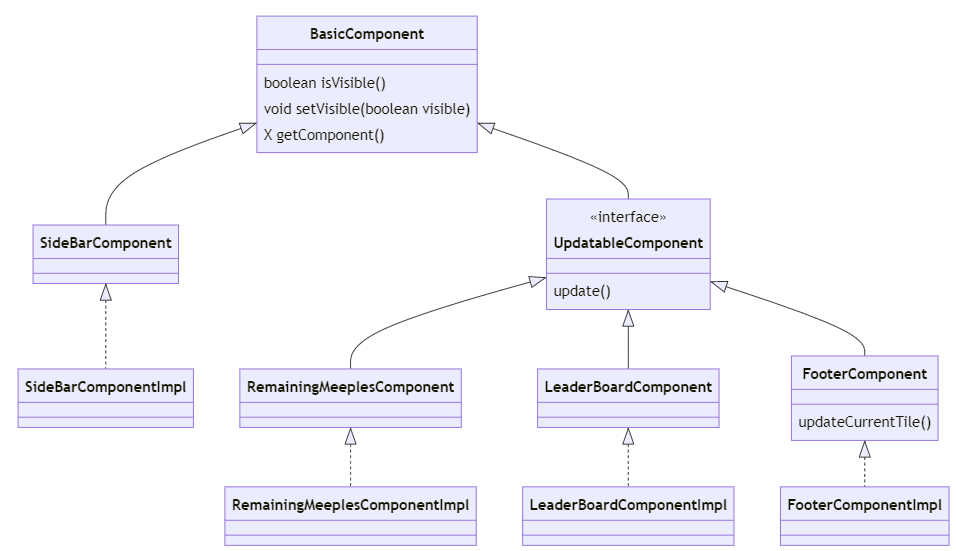
\includegraphics[scale=0.70]{images/HUD_uml2.png}
    \caption{Rappresentazione UML dei componenti grafici della HUD}
\end{figure}

\paragraph{Problema:}
è necessaria la creazione di una HUD che permetta al giocatore di compiere azioni all'interno del tabellone e visualizzarne i dati di gioco

\paragraph{Soluzione:}
Per garantire il single responsability sono stati creati 4 componenti principali:
\begin{itemize}
    \item RemainingMeepleComponent per la visualizzazione dei propri seguaci rimanenti
    \item LeaderBoardComponent per la visualizzazione la classifica dei giocatori 
    \item SideBarComponent per la gestione del tabellone di gioco
    \item FooterComponent per la visualizzazione dei dati di gioco
\end{itemize}

è stata utilizzata uno strategy pattern che vede un'interfaccia BasicComponent al vertice e che permette già l'implementazione di componenti con nessuna particolare necessità come SideBarComponent, unicamente utilizzato per l'inserimento in input dei comandi da parte dei giocatori. I restanti componenti dovendo invece mostrare dati di gioco hanno necessitato della funzione update(), ricavata dall'interfaccia UpdatableComponent che ha esteso BasicComponent.

Da notare come LeaderBoardComponent, per esempio, sia un componente a se stante e quindi ottimo per essere utilizzato in altri contesti di view, per esempio come in gameOverScene.
\clearpage


